\section{Contribution}
There are many ways to contribute an open source project. Most of new users start reporting and help to verify bugs. More advanced user help to improve documentation and try to help others solving issues. It is also common to share configuration which solve a special problem in the network management domain.

If you are a developer and you would like contribute source code to fix a bug or make an enhancement in OpenNMS, you have to sign the \emph{OpenNMS Contributor Agreement}. It allows \textit{The OpenNMS Group, Inc.} to publish your code contribution under GPLv3+. You can find the agreement at the following link \url{http://www.opennms.org/wiki/Contributor_Agreement}. 

\subsection*{Where can I start with the source code}
The source code is hosted on \emph{GitHub}\footnote{\url{http://www.github.com}}. 
Code contributions can be merged into \emph{OpenNMS} with \emph{pull requests}. The workflow to get your source code into \emph{OpenNMS} is shown in picture \ref{fig:contrib-workflow} on page \pageref{fig:contrib-workflow}.
\begin{figure}
	\centering
	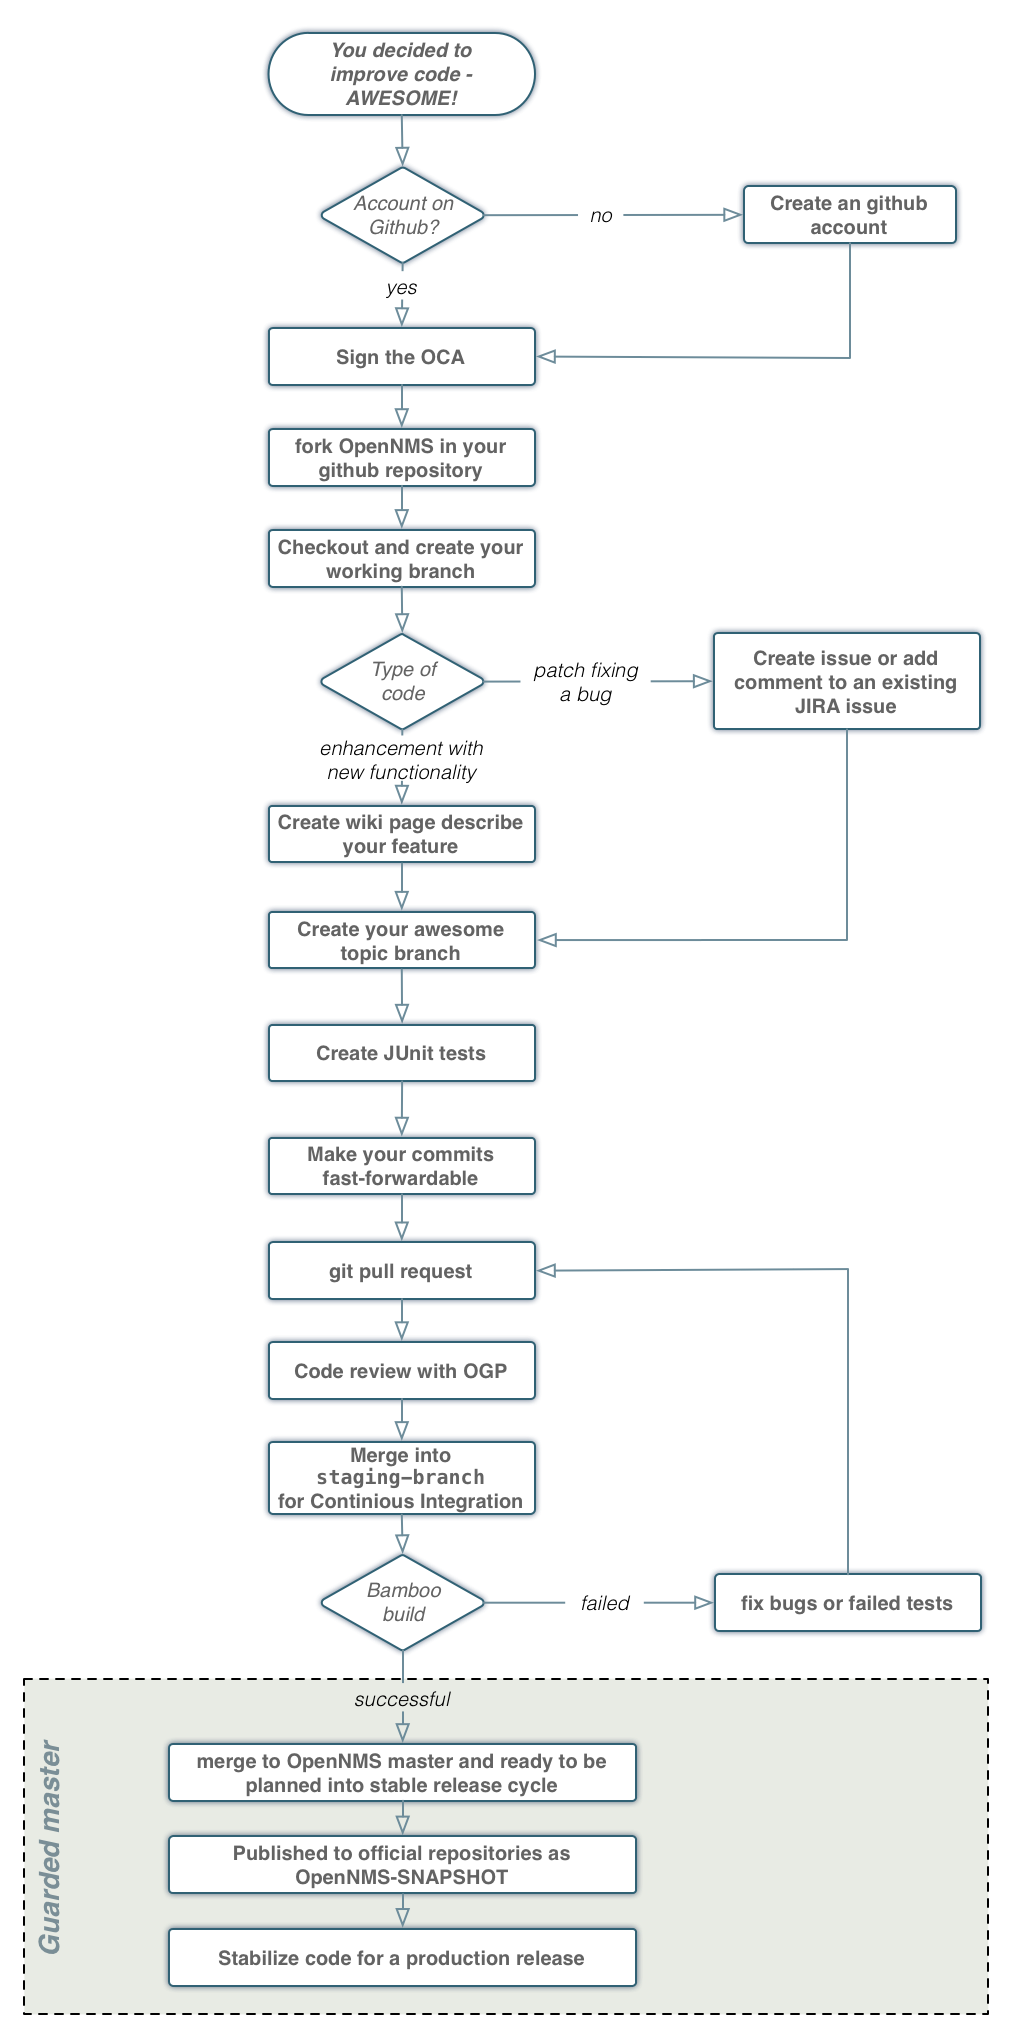
\includegraphics[width=0.75\textwidth]{images/contribution-workflow.png}
	\caption{Workflow for code contribution}
	\label{fig:contrib-workflow}
\end{figure}

\subsection*{Get your IDE up and running}
The \emph{OpenNMS} project is written in \emph{Java}. To maintain and handle external libraries it uses \emph{Maven}. It contains even more advanced technologies like \emph{OSGi} for class loading and \emph{Vaadin} as user interface framework. As version control system the project uses \emph{git}. To get an introduction working with \emph{git} and get your development environment up and running you can find documentation on the following wiki pages:
\begin{itemize}
  \item \url{http://www.opennms.org/wiki/Developing_with_Git}
  \item \url{http://www.opennms.org/wiki/Eclipse_and_OpenNMS}
\end{itemize}

